\section{Metriche di Valutazione}
In questa sezione vengono analizzate le prestazioni dei modelli attraverso i grafici delle principali metriche di valutazione: ROUGE, WER, cosine similarity e BERTScore.\\
Inoltre è stata anche utilizzata la metrica personalizzata \texttt{myevaluation}, che verrà approfondita in seguito.\\ 
Queste metriche sono state scelte per misurare in modo accurato la qualit\`a dei riassunti generati, confrontandoli con quelli di riferimento.\\
Le valutazioni sono state effettuate utilizzando il dataset di test, che non \`e stato utilizzato durante l'addestramento del modello.\\
Durante la fase di inferenza, sono stati generati 1000 riassunti a partire dai dati di test per ogni istanza di ogni classe di modelli e sono stati confrontati con i riassunti di riferimento.\\

\subsection{ROUGE (Recall-Oriented Understudy for Gisting Evaluation)}
Sono state calcolate tre varianti di ROUGE:
\begin{itemize}
    \item ROUGE-1: confronta unigrammi tra il riassunto generato e quello di riferimento
    \item ROUGE-2: considera bigrammi per valutare la similarit\`a tra i due testi
    \item ROUGE-L: confronta la sottosequenza pi\`u lunga comune tra i due testi
\end{itemize}    

I grafici nella Figura \ref{fig:rouge_comparison} confrontano le performance in termini di ROUGE-1, ROUGE-2 e ROUGE-L per i quattro modelli. Il modello Seq2SeqBiLSTM mostra un miglioramento nei punteggi ROUGE rispetto al Seq2SeqLSTM e al Seq2SeqLSTMGlove, indicando una maggiore capacit\`a di catturare similarit\`a lessicali.
\begin{figure}[H]
    \centering
    \rougeonesubimg{0.45}{Seq2SeqLSTM}{rouge1_seq2seq_lstm}
    \hfill
    \rougeonesubimg{0.45}{Seq2SeqBiLSTM}{rouge1_seq2seq_bilstm}
    \hfill
    \rougeonesubimg{0.45}{Seq2Seq3BiLSTM}{rouge1_seq2seq_3bilstm}
    \hfill
    \rougeonesubimg{0.45}{Seq2SeqLSTMGlove}{rouge1_seq2seq_lstm_glove}
    \hfill

    \rougetwosubimg{0.45}{Seq2SeqLSTM}{rouge2_seq2seq_lstm}
    \hfill
    \rougetwosubimg{0.45}{Seq2SeqBiLSTM}{rouge2_seq2seq_bilstm}
    \hfill
    \rougetwosubimg{0.45}{Seq2Seq3BiLSTM}{rouge2_seq2seq_3bilstm}
    \hfill
    \rougetwosubimg{0.45}{Seq2SeqLSTMGlove}{rouge2_seq2seq_lstm_glove}
    \hfill

    \rougelubimg{0.45}{Seq2SeqLSTM}{rougeL_seq2seq_lstm}
    \hfill
    \rougelubimg{0.45}{Seq2SeqBiLSTM}{rougeL_seq2seq_bilstm}
    \hfill
    \rougelubimg{0.45}{Seq2Seq3BiLSTM}{rougeL_seq2seq_3bilstm}
    \hfill
    \rougelubimg{0.45}{Seq2SeqLSTMGlove}{rougeL_seq2seq_lstm_glove}
    \hfill

    \caption{Confronto dei punteggi ROUGE tra i modelli Seq2SeqLSTM, Seq2SeqBiLSTM, Seq2Seq3BiLSTM, Seq2SeqLSTMGlove.}
    \label{fig:rouge_comparison}
\end{figure}

\subsection{WER (Word Error Rate)}
Il WER \`e una metrica che calcola il tasso di errore tra due sequenze di parole.\\
In particolare, il WER calcola il numero di operazioni di inserimento, cancellazione e sostituzione necessarie per trasformare una sequenza di parole in un'altra.\\

Il confronto del WER, mostrato nella Figura \ref{fig:wer_comparison}, evidenzia che il modello Seq2SeqBiLSTM ottiene risultati migliori, indicando una maggiore accuratezza nella generazione delle parole.

\begin{figure}[H]
    \centering
    \wersubimg{0.45}{Seq2SeqLSTM}{wer_seq2seq_lstm}
    \hfill
    \wersubimg{0.45}{Seq2SeqBiLSTM}{wer_seq2seq_bilstm}
    \hfill
    \wersubimg{0.45}{Seq2Seq3BiLSTM}{wer_seq2seq_3bilstm}
    \hfill
    \wersubimg{0.45}{Seq2SeqLSTMGlove}{wer_seq2seq_lstm_glove}
    
    \caption{Confronto del Word Error Rate tra i modelli Seq2SeqLSTM, Seq2SeqBiLSTM, Seq2Seq3BiLSTM, Seq2SeqLSTMGlove.}
    \label{fig:wer_comparison}
\end{figure}


\subsection{Cosine Similarity}
La similarit\`a cosenica \`e una metrica che calcola la similarit\`a tra due vettori in uno spazio multidimensionale.\\
Nel caso specifico della generazione di riassunti, la similarit\`a cosenica \`e stata calcolata tra i vettori di embedding delle parole nei riassunti generati e quelli nei riassunti di riferimento, con il fine di valutare la qualit\`a dei riassunti generati.\\
La Figura \ref{fig:cosine_similarity_comparison} confronta i valori di similarit\`a cosenica. Anche in questo caso, il modello Seq2SeqBiLSTM ottiene valori pi\`u alti, suggerendo una maggiore correlazione semantica con i riassunti di riferimento.

\begin{figure}[H]
    \centering
    \cssubimg{0.45}{Seq2SeqLSTM}{cs_seq2seq_lstm}
    \hfill
    \cssubimg{0.45}{Seq2SeqBiLSTM}{cs_seq2seq_bilstm}
    \hfill
    \cssubimg{0.45}{Seq2Seq3BiLSTM}{cs_seq2seq_3bilstm}
    \hfill
    \cssubimg{0.45}{Seq2SeqLSTMGlove}{cs_seq2seq_lstm_glove}
    
    \caption{Confronto della cosine similarity tra i modelli Seq2SeqLSTM, Seq2SeqBiLSTM, Seq2Seq3BiLSTM, Seq2SeqLSTMGlove.}
    \label{fig:cosine_similarity_comparison}
\end{figure}

\subsection{BERTScore}
Il BERTScore \`e una metrica che utilizza il modello BERT per calcolare la similarit\`a tra due testi.\\
In particolare, il BERTScore calcola la similarit\`a tra i vettori di embedding delle parole nei riassunti generati e quelli nei riassunti di riferimento, tenendo conto del contesto semantico delle parole.\\
La Figura \ref{fig:bert_score_comparison} mostra i valori di BERTScore per i diversi modelli. Anche in questo caso, il modello Seq2SeqBiLSTM ottiene risultati migliori, suggerendo una maggiore capacit\`a di catturare la similarit\`a semantica tra i riassunti generati e quelli di riferimento.

\begin{figure}[H]
    \centering
    \bertsubimg{0.45}{Seq2SeqLSTM}{bert_seq2seq_lstm}
    \hfill
    \bertsubimg{0.45}{Seq2SeqBiLSTM}{bert_seq2seq_bilstm}
    \hfill
    \bertsubimg{0.45}{Seq2Seq3BiLSTM}{bert_seq2seq_3bilstm}
    \hfill
    \bertsubimg{0.45}{Seq2SeqLSTMGlove}{bert_seq2seq_lstm_glove}
    
    \caption{Confronto del BERTScore tra i modelli Seq2SeqLSTM, Seq2SeqBiLSTM, Seq2Seq3BiLSTM, Seq2SeqLSTMGlove.}
    \label{fig:bert_score_comparison}
\end{figure}

\subsection{My Evaluation}
La metrica \texttt{myevaluation} \`e stata progettata per valutare la qualit\`a dei riassunti generati in modo pi\`u dettagliato.\\
Essa tiene conto di diversi fattori e ciuscuno di essi ha uno specifico peso in base alla sua importanza.\\
La formula con cui viene calcolata la metrica \texttt{myevaluation} \`e la seguente:
\[
    \texttt{MyEval} = cs\_PS\_OS \cdot W_{cs\_PS\_OS} + keyword\_overlap \cdot W_{keyword\_overlap} + bert\_score \cdot W_{bert\_score}
\]
Dove:
\begin{itemize}
    \item $cs\_PS\_OS$ \`e la similarit\`a cosenica tra il riassunto generato e quello originale
    \item $keyword\_overlap$ \`e la percentuale di parole chiave presenti nel riassunto generato rispetto a quelle nel riassunto originale
    \item $bert\_score$ \`e il punteggio BERTScore tra il riassunto generato e quello originale
    \item $W_{cs\_PS\_OS}$, $W_{keyword\_overlap}$ e $W_{bert\_score}$ sono i pesi associati a ciascun fattore
\end{itemize}

La Figura \ref{fig:myevaluation_comparison} mostra i risultati della metrica \texttt{myevaluation} per i diversi modelli.\\
Il modello Seq2SeqBiLSTM ottiene i punteggi pi\`u alti, suggerendo una qualit\`a superiore dei riassunti generati rispetto agli altri modelli.
\begin{figure}[H]
    \centering
    \myevalsubimg{0.45}{Seq2SeqLSTM}{myeval_seq2seq_lstm}
    \hfill
    \myevalsubimg{0.45}{Seq2SeqBiLSTM}{myeval_seq2seq_bilstm}
    \hfill
    \myevalsubimg{0.45}{Seq2Seq3BiLSTM}{myeval_seq2seq_3bilstm}
    \hfill
    \myevalsubimg{0.45}{Seq2SeqLSTMGlove}{myeval_seq2seq_lstm_glove}
    
    \caption{Confronto della metrica \texttt{myevaluation} tra i modelli Seq2SeqLSTM, Seq2SeqBiLSTM, Seq2Seq3BiLSTM, Seq2SeqLSTMGlove.}
    \label{fig:myevaluation_comparison}
\end{figure}

\subsection{Confronto tra le Architetture}
Di seguito viene riportata una tabella comparativa (figura \ref{fig:models_comparison_instances}) tra i vari modelli implementati, con i rispettivi risultati ottenuti al termine dell'addestramento.\\
Per ogni classe di modelli sono stati effettuati numerosi tentativi e test, riportati in seguito in una tabella comparativa le varie istanze di configurazione e i risultati ottenuti.\\
Possiamo subito notare che il modello Seq2SeqBiLSTM ha ottenuto i risultati migliori in quasi tutte le metriche.
\begin{figure}[H]
    \centering
    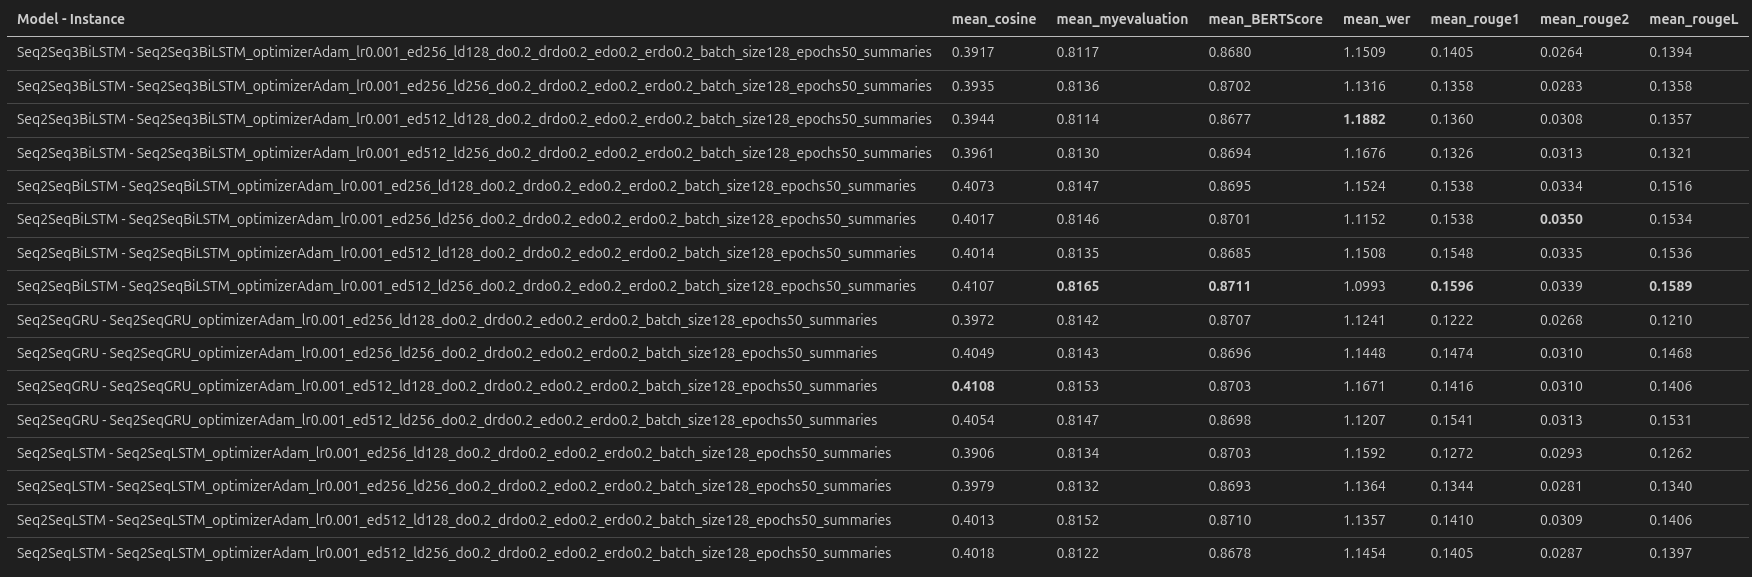
\includegraphics[width=1\textwidth]{media/models_comparison_instances.png}
    \caption{Comparazione delle istanze dei modelli}
    \label{fig:models_comparison_instances}
\end{figure}
  
